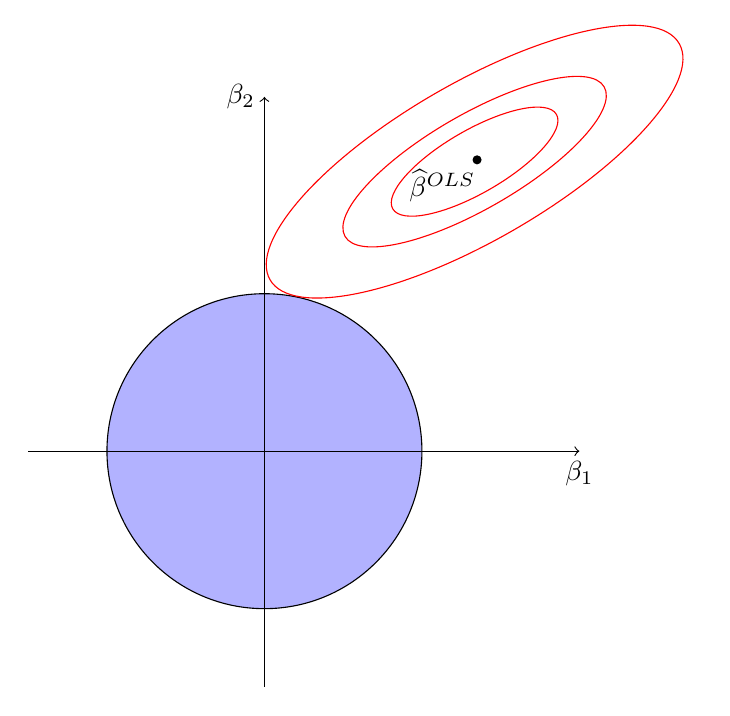
\begin{tikzpicture}
\draw [fill] (2.7,3.7) circle [radius=0.05];
\node [below left] (a) at (2.8,3.7) {$\widehat{\boldsymbol{\beta}}^\text{OLS}$};
\draw (0,0) circle (2cm) [fill= blue!30];
\draw [<-] (0,4.5) node [left] {$\beta_2$}-- (0,-3);
\draw[<-] (4,0) node [below] {$\beta_1$} -- (-3,0);
\begin{scope}[rotate = 30, red]
\clip[draw] (4.15,1.85) ellipse (3cm and 1cm);
\clip[draw] (4.15,1.85)ellipse (1.9 cm and 0.6 cm); 
\clip[draw] (4.15,1.85) ellipse (1.2 cm and 0.4 cm);
\end{scope}
\end{tikzpicture}